%%%%%%%%%%%%%%%%%%%%%%%%%%%%%%%%%%%%%%%%%
% Simple Sectioned Essay Template
% LaTeX Template
%
% This template has been downloaded from:
% http://www.latextemplates.com
%
% Note:
% The \lipsum[#] commands throughout this template generate dummy text
% to fill the template out. These commands should all be removed when 
% writing essay content.
%
%%%%%%%%%%%%%%%%%%%%%%%%%%%%%%%%%%%%%%%%%

%----------------------------------------------------------------------------------------
%	PACKAGES AND OTHER DOCUMENT CONFIGURATIONS
%----------------------------------------------------------------------------------------

\documentclass[12pt]{article}

\usepackage[italian]{babel}
\usepackage[utf8]{inputenc}
\usepackage{geometry}
\usepackage{graphicx}
\usepackage{float}
\usepackage{wrapfig}
\usepackage[dvipsnames]{xcolor}
\usepackage{acronym}
\usepackage{lipsum}
\usepackage{listings}
\usepackage{mathtools}

\geometry{a4paper}

\linespread{1.1}

\graphicspath{{img/}}

\definecolor{back}{rgb}{1,0.93,0.76} 
\lstset{ %
	backgroundcolor=\color{back},  % choose the background color; you must add \usepackage{color} or \usepackage{xcolor}; should come as last argument
	basicstyle=\tiny,        		% the size of the fonts that are used for the code
	breakatwhitespace=false,        % sets if automatic breaks should only happen at whitespace
	breaklines=true,                % sets automatic line breaking
	captionpos=b,                   % sets the caption-position to bottom
	commentstyle=\color{gray},   	% comment style
	frame=single,	                % adds a frame around the code
	keepspaces=true,                % keeps spaces in text, useful for keeping indentation of code (possibly needs columns=flexible)
	keywordstyle=\color{blue},      % keyword style
	language=Python,               	% the language of the code
	numbers=none,                   % where to put the line-numbers; possible values are (none, left, right)
	numbersep=5pt,                  % how far the line-numbers are from the code
	numberstyle=\tiny\color{black}, % the style that is used for the line-numbers
	rulecolor=\color{black},        % if not set, the frame-color may be changed on line-breaks within not-black text (e.g. comments (green here))
	showspaces=false,               % show spaces everywhere adding particular underscores; it overrides 'showstringspaces'
	showstringspaces=false,         % underline spaces within strings only
	showtabs=false,                 % show tabs within strings adding particular underscores
	stepnumber=1,                   % the step between two line-numbers. If it's 1, each line will be numbered
	stringstyle=\color{OrangeRed},  % string literal style
	tabsize=2                   	% sets default tabsize to 2 spaces
}

\acrodef{PCA}{\emph{Principal Component Analysis}}

\newcommand{\codice}[2]{\lstinputlisting[firstline=#1, lastline=#2]{code/PCA.py}}

\begin{document}

%----------------------------------------------------------------------------------------
%	TITLE PAGE
%----------------------------------------------------------------------------------------

\begin{titlepage}

\newcommand{\HRule}{\rule{\linewidth}{0.5mm}}

\center

\textsc{\LARGE Università degli studi di Firenze}\\[1.5cm]
\textsc{\Large Corso di Laurea Magistrale in Informatica}\\[0.5cm]
\textsc{\large Multivariate Analysis and Statistical Learning}\\[0.5cm]

\HRule \\[0.4cm]
{ \huge \bfseries Principal Component Analysis: dalla teoria alla pratica}\\[0.4cm]
\HRule \\[1.5cm]

\begin{minipage}{0.4\textwidth}
\begin{flushleft} \large
\emph{Autore:}\\
Marco \textsc{Buracchi}
\end{flushleft}
\end{minipage}
~
\begin{minipage}{0.4\textwidth}
\begin{flushright} \large
\emph{Docente:} \\
Prof.ssa Anna \textsc{Gottard}
\end{flushright}
\end{minipage}\\[4cm]

{\large \today}\\[3cm] % Date, change the \today to a set date if you want to be precise
\vfill % Fill the rest of the page with whitespace

\end{titlepage}

%----------------------------------------------------------------------------------------
%	TABLE OF CONTENTS
%----------------------------------------------------------------------------------------
\tableofcontents
\newpage
%----------------------------------------------------------------------------------------
%	TESTO
%----------------------------------------------------------------------------------------

\section{Principal Component Analysis}

	La \ac{PCA} è una trasformazione lineare della matrice dei dati il cui scopo è rappresentare la variazione presente nelle tante variabili utilizzando un numero k molto più piccolo di \emph{“fattori”} o \emph{“componenti principali”}. Si costruisce un nuovo spazio su cui rappresentare i campioni	ridefinendo gli assi utilizzando le componenti principali al posto delle variabili originali. L’uso di questi nuovi assi permette di rappresentare la vera natura multivariata dei dati in un numero relativamente piccolo di dimensioni e di usare questa rappresentazione per identificare la struttura dei dati stessi.  
	
	\subsection{Cosa fa?}
		Supponiamo di aver misurato il valore di due variabili su 40 campioni come in Figura \ref{fig:plot1} 
		\begin{figure}[H]
			\begin{center}
				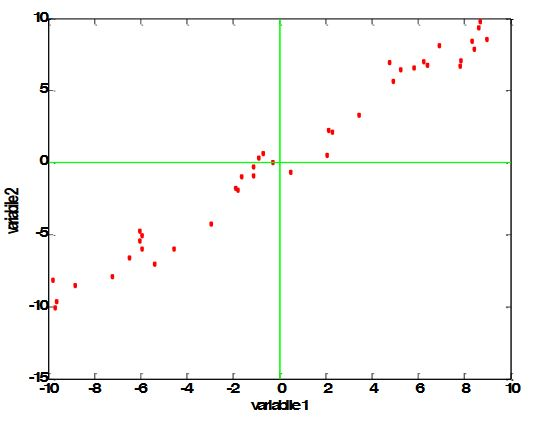
\includegraphics[scale=.5]{plotTeoria}
				\caption{Plot variabili A e B}
				\label{fig:plot1}
			\end{center}
		\end{figure}
		Vogliamo studiare le relazioni tra i campioni. Le distanze tra i campioni sono usate per definire similarità e differenze. In altre parole, lo scopo della \ac{PCA} è di descrivere le distanze fra i punti (distribuzione, variabilità) utilizzando il minor numero di dimensioni possibili. Questo scopo si raggiunge costruendo assi che si allineano coi dati. Come si vede dal grafico nessuna delle variabili originali descrive completamente la variabilità all’interno dei dati stessi. 
		\begin{figure}[H]
			\begin{center}
				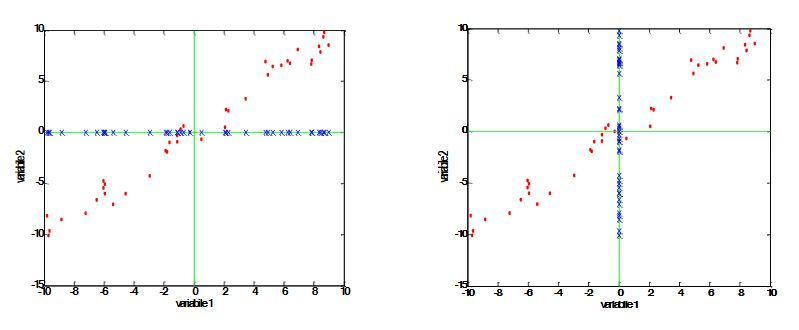
\includegraphics[scale=.6]{proiezione}
				\caption{Proiezione variabili A e B}
				\label{fig:proiezione}
			\end{center}
		\end{figure}
		Se prendiamo come componenti principali però, le linee blu in figura \ref{fig:componenti}, la prima componente principale descrive una quantità della variabilità originale maggiore di quella spiegata da ciascuna delle due variabili prese singolarmente. Essa spiega la massima percentuale della variabilità presente nei dati rappresentabile in una sola dimensione. Questa percentuale di variabilità spiegata può essere calcolata attraverso la varianza. La varianza è infatti un indice della dispersione dei dati lungo una particolare direzione ed è indipendente dal sistema di riferimento: una rotazione degli assi mantiene inalterata la varianza totale all’interno dei dati. 
		\begin{figure}[H]
			\begin{center}
				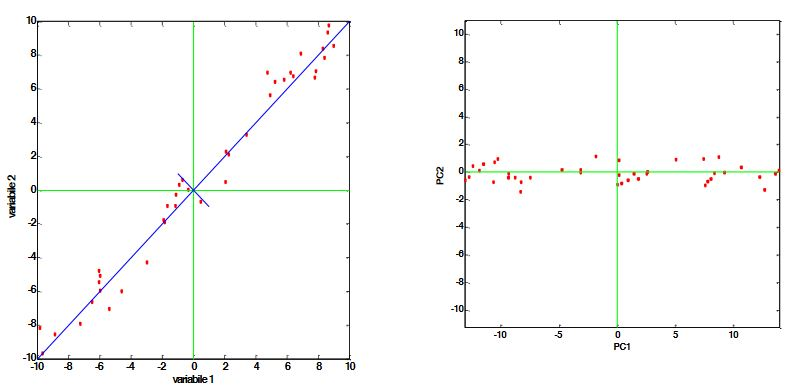
\includegraphics[scale=.6]{componenti}
				\caption{Componenti principali}
				\label{fig:componenti}
			\end{center}
		\end{figure}
		In questo esempio, la prima componente principale cattura praticamente tutta la variabilità presente nei dati (99.83\%) mentre la seconda descrive la rimanente variazione (0.17\%). Questa considerazione può essere generalizzata: le componenti principali successive spiegano una sempre minore percentuale della variabilità originale. Seguendo questo principio è possibile dire che le ultime componenti principali descrivono principalmente \emph{rumore}.
		
	\subsection{Come funziona?}
			
		\begin{description}
			\item[Standardizzazione:] \hfill \\
			 Standardizziamo i dati (media = 0 e varianza = 1). In questo modo possiamo lavorare con variabili che hanno scale e unità di misura differenti.
			\item[Calcolo della covarianza/correlazione:] \hfill \\
			Calcoliamo la matrice $\mathcal{S}$ di covarianza. La covarianza di due variabili indica quanto le due variabili si influenzino a vicenda.
			$$\mathcal{S} = \frac{1}{n-1} \sum_{1}^{n} (x-\mu)(x-\mu)^T$$
			In alternativa possiamo utilizzare anche la matrice di correlazione.
			\item[Calcolo autovalori/autovettori:] \hfill \\ 
			Calcoliamo gli autovalori e gli autovettori della matrice di covarianza. Per definizione $$\mathcal{S} \times v = \lambda \times v$$
			
			Ognuno di questi autovettori corrisponde ad un autovalore la cui grandezza indica quanta varianza viene spiegata da quell'autovettore. Ordiniamo quindi gli autovalori in ordine decrescente e prendiamo i primi k. Chiamiamo $\mathcal{V}$ la matrice degli autovettori risultante.
			\item[Ruotiamo i dati:] \hfill \\
			Per convertire le osservazioni nel nuovo sistema di assi, moltiplichiamo i dati originali per gli autovettori che indicano la direzione dei nuovi assi (componenti principali). Questi dati ruotati vengono chiamati \emph{score}. $$Sc = X \times \mathcal{V}$$
			\item[Dati ridotti:] \hfill \\
			A questo punto è possibile utilizzare i nuovi dati.
		\end{description}
	
\section{Implementazione Python}

	Passiamo adesso all'implementazione di un piccolo esempio di \ac{PCA} sul dataset \emph{IRIS}. Per questa realizzazione è stato scelto il linguaggio \emph{Python} con la relativa libreria \emph{pandas}.

	\subsection{PANDAS}

		pandas è una libreria Python open-source, ad alte prestazioni e con licenza BSD che fornisce strutture dati e strumenti per l'analisi facili da usare.
		\begin{wrapfigure}{l}{0.3\textwidth} % Inline image example
			\begin{center}
				
\includegraphics[width=0.28\textwidth]{numFocus.png}
			\end{center}
		\end{wrapfigure}
		\`{E} un progetto sponsorizzato da NumFocus. Questo assicura lo sviluppo continuo e a livello mondiale e permette anche di aiutare gli sviluppatori con donazioni o citazioni.Permette di lavorare con dati organizzati in maniera \emph{relazionale} o \emph{etichettata} in maniera intuitiva. Le sue due strutture dati principali sono le serie (unidimensionali) e i dataframe (bidimensionali). Per il nostro esempio utilizzeremo questa seconda struttura.
		

	\subsection{Implementazione}
	
		Come già detto, utilizzeremo il dataset IRIS che contiene 150 misurazioni di fiori iris di tre specie diverse. La figura \ref{fig:iris} schematizza le variabili del dataset che sono:
		\begin{enumerate}
			\item Larghezza dei sepali in cm
			\item Lunghezza dei sepali in cm
			\item Larghezza dei petali in cm
			\item Lunghezza dei petali in cm
			\item Specie (setosa,versicolor,virginica)
		\end{enumerate}
		\begin{figure}
			\begin{center}
				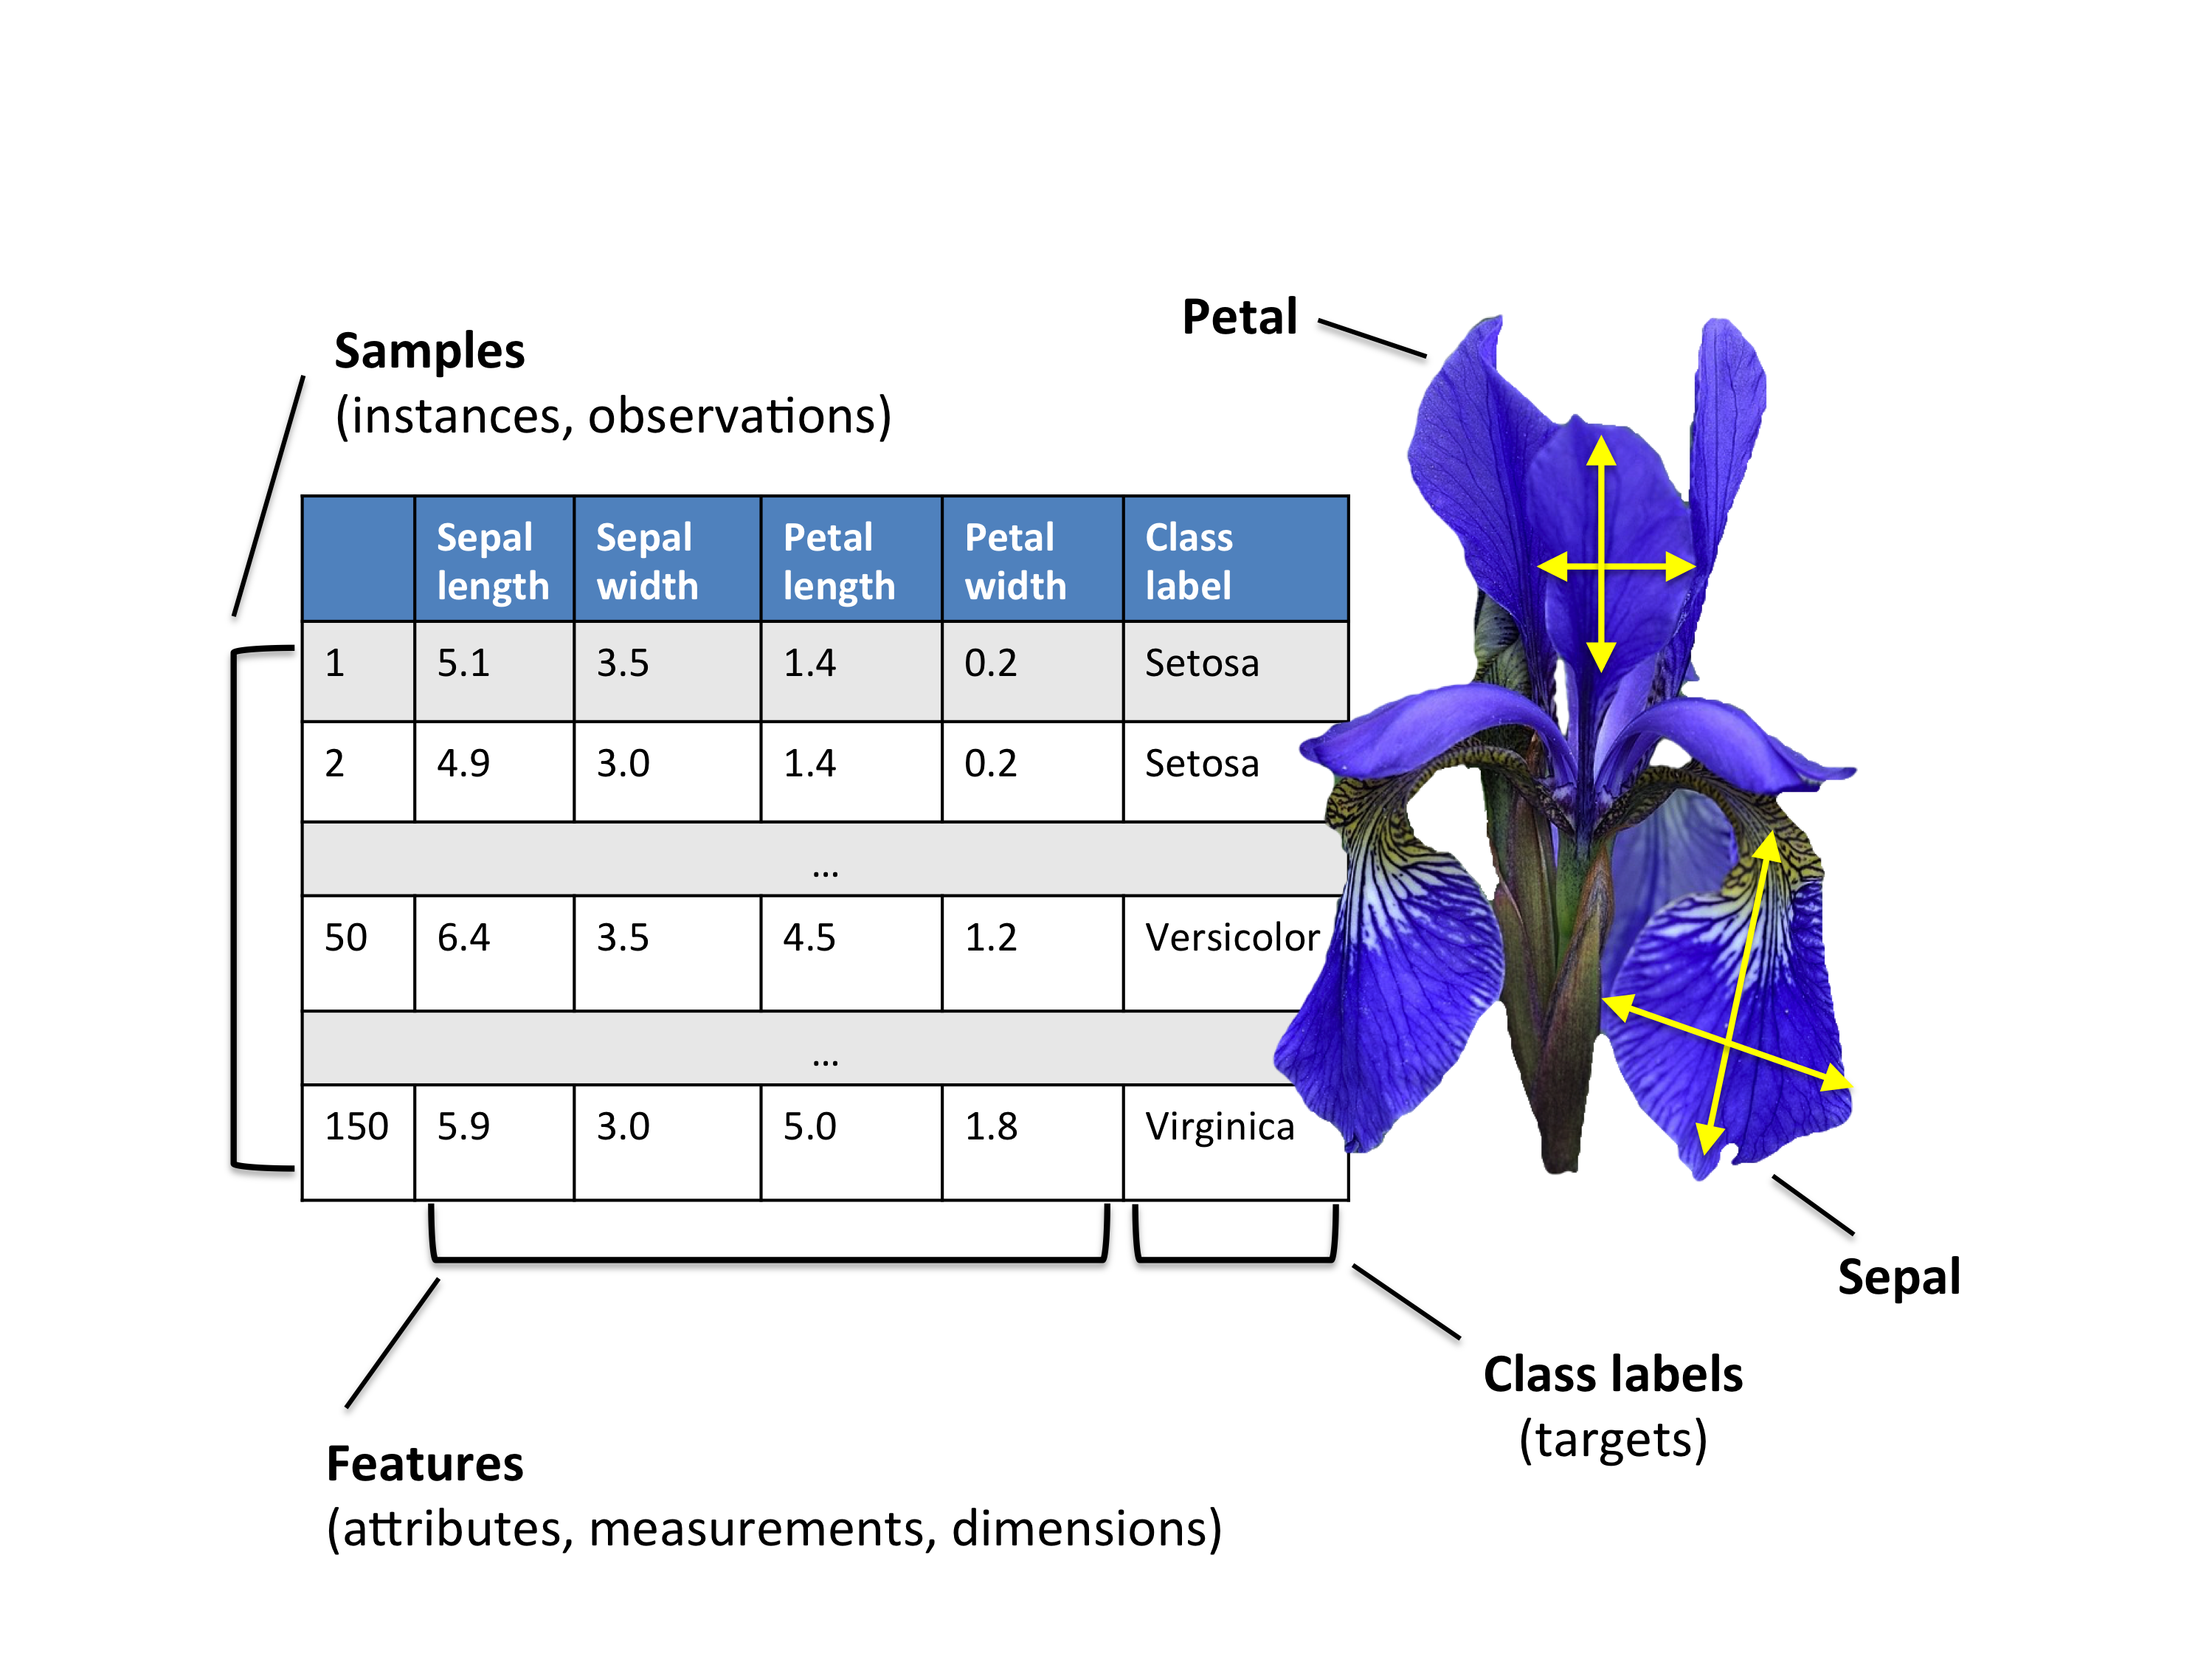
\includegraphics[scale=.1]{iris}
				\caption{Struttura dataset}
				\label{fig:iris}
			\end{center}
		\end{figure}

		\subsubsection{Preparazione dataset}

			\begin{description}

				\item[Caricamento dataset] \hfill \\
				Come prima cosa, scarichiamo il dataset dall'archivio della UCI (Università della California) e carichiamolo assegnando i nomi desiderati alle colonne e rimuovendo i valori NA.
				
				\lstinputlisting[firstline=16, lastline=25]{code/PCA.py}
				
				\begin{figure}[H]
					\begin{center}
						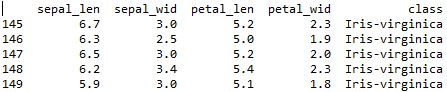
\includegraphics[scale=.7]{tab}
						\caption{Dataset memorizzato}
						\label{fig:dataset}
					\end{center}
				\end{figure}
				
				Dopo questi comandi otteniamo il risultato visibile in figura \ref{fig:dataset}. Dividiamo i valori numerici dalla specie creando una matrice $X \in \mathcal{M}^{150x4}$ e un vettore $y \in \mathcal{M}^{150x1}$
				
				\codice{30}{32}
				
				\item[Analisi descrittiva] \hfill \\
				Per avere un'idea di come si distribuiscono le tre classi di fiori sulle varie caratteristiche, creiamo qualche istogramma.				
				\codice{37}{56}				
				\begin{figure}
					\begin{center}
						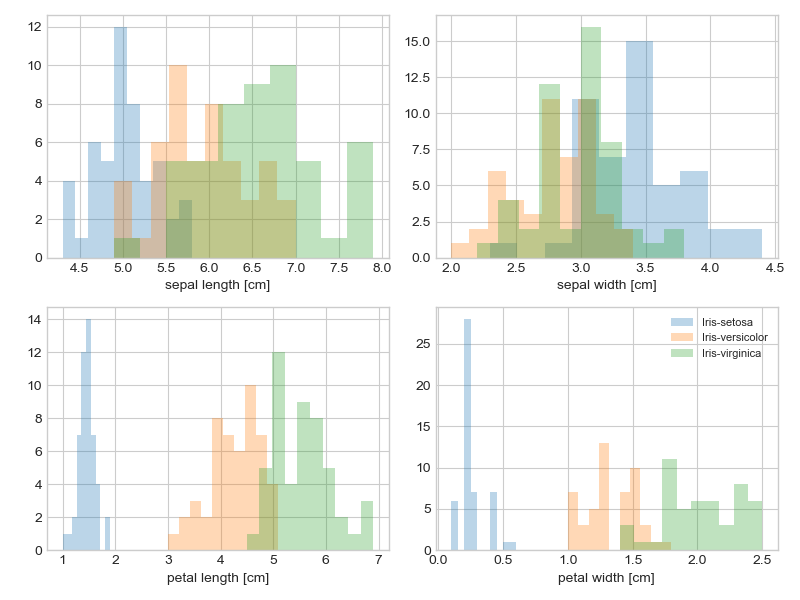
\includegraphics[scale=.5]{isto}
						\caption{Analisi descrittiva}
						\label{fig:isto}
					\end{center}
				\end{figure}				
				Il risultato è visibile in figura \ref{fig:isto}
							
				\item[Standardizzazione] \hfill \\
				Standardizziamo i dati in scala unitaria (media = 0 e varianza = 1) per migliorare le performance.
				\codice{58}{59}
			\end{description} 
		
		\subsubsection{Calcolo autovalori e autovettori}
		
			Calcoliamo gli autovettori e gli autovalori della matrice di covarianza e della matrice di correlazione. Possiamo calcolarli utilizzando la formula teorica, utilizzando una funzione di libreria oppure applicando la decomposizione a valori singolari. In ogni caso, i risultati saranno gli stessi (tranne nel caso della SVD che differisce solo per alcuni segni dato che la scomposizione è unica a meno di matrici di fase).
			\codice{61}{94}
			La matrice che si ottiene è la seguente:
			$$\begin{bmatrix}
				0.52237162 & -0.37231836 & -0.72101681 & 0.26199559\\
				-0.26335492 & -0.92555649 & 0.24203288 & -0.12413481\\
				0.58125401 & -0.02109478 & 0.14089226 & -0.80115427\\
				0.56561105 & -0.06541577 & 0.6338014 & 0.52354627\\
			\end{bmatrix}$$
			
		\subsubsection{Selezione delle componenti}		
			Vogliamo ridurre le dimensioni dello spazio delle variabili proiettandolo in un sottospazio più piccolo. I suoi assi saranno gli autovettori appena calcolati. Purtroppo, in questo momento definiscono solamente la direzione perché sono tutti a lunghezza unitaria.	Per stabilire quale può essere abbandonato senza perdere troppa informazione controlliamo ed ordiniamo i rispettivi autovalori.
			\codice{96}{105}
			A questo punto calcoliamo la varianza spiegata delle singole componenti e mostriamola in un grafico (Figura \ref{fig:varSpieg}).
			\codice{108}{123}
			\begin{figure}
				\begin{center}
					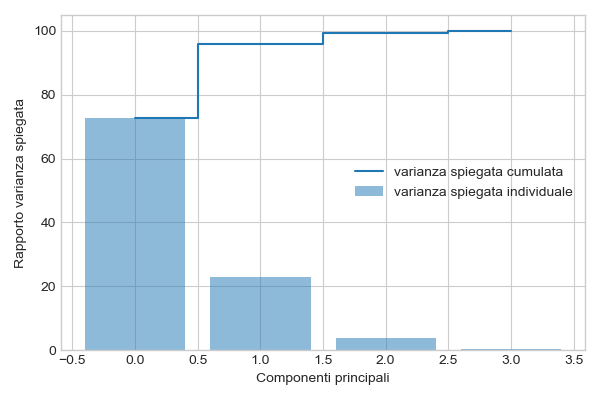
\includegraphics[scale=.5]{istoVarianza}
					\caption{Varianza spiegata}
					\label{fig:varSpieg}
				\end{center}
			\end{figure}
			Dal grafico possiamo dedurre che la maggior parte della varianza può essere spiegata dalla prima componente (72.77\%). Anche la seconda porta un po' di informazione (23.03\%) mentre la terza e la quarta possono tranquillamente essere rimosse senza perdere troppa informazione.
			
		\subsubsection{Matrice di proiezione}
			Per costruire la matrice di proiezione che ci permetterà di passare da uno spazio 4-dimensionale ad uno 2-dimensionale concateniamo le prime due componenti degli autovettori.
			\codice{125}{127}
			La matrice risultante sarà quindi:
			$$W = \begin{bmatrix}
				0.52237162 & -0.37231836\\
				-0.26335492 & -0.92555649\\
				0.58125401 & -0.02109478\\
				0.56561105 & -0.06541577\\
			\end{bmatrix}$$
			
		\subsubsection{Proiezione nel nuovo spazio}
			Come ultimo passo, utilizzeremo la matrice $W$ per trasformare i nostri campioni nel nuovo sottospazio con l'equazione $$Y = X\times W \qquad Y \in \mathcal{M}^{150x2}$$
			\codice{132}{133}
			Dopo l'applicazione della \ac{PCA} otteniamo uno spazio bidimensionale dove i campioni sono distribuiti lungo i nuovi assi (Figura \ref{img:PCA}).
			\begin{figure}
				\begin{center}
					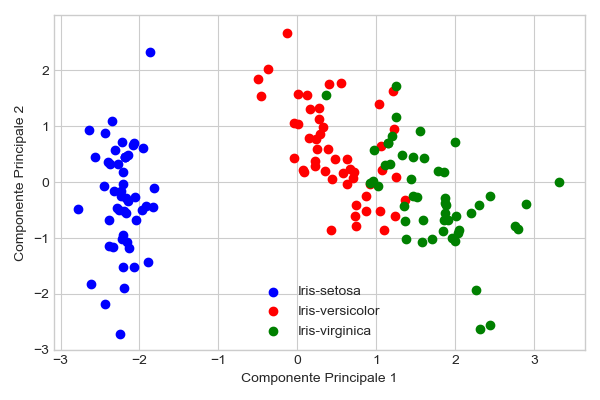
\includegraphics[scale=.5]{PCA}
					\caption{Distribuzione campioni dopo PCA}
					\label{img:PCA}
				\end{center}
			\end{figure}
			
			Esiste anche una funzione di libreria che calcola direttamente dal dataset la \ac{PCA} con il numero di componenti scelto.
			\codice{149}{151}
			
\section{Caso di studio}
	L'enorme diffusione di sistemi informatici connessi tramite dispositivi di telecomunicazione ha aumentato in maniera esponenziale il problema della sicurezza delle reti. Purtoppo i dati sul traffico di rete raccolti per l'analisi delle intrusioni hanno in genere molte dimensioni che rendono difficile sia l'analisi che la semplice visualizzazione. La \ac{PCA} viene utilizzata per ridurre il numero di variabili dai campioni misurati per consentire analisi del traffico e visualizzazioni più semplici.
	
	\subsection{Il problema}
		Negli anni, per contrastare il sempre maggior numero di compromissioni di sistemi informatici da parte di utenti malintenzionati (vedi ad esempio i molti casi di documenti, filmati, foto o informazioni personali rubati da servizi cloud) sono stati sviluppati Sistemi di Rilevamento delle Intrusioni (IDS) sempre più sofisticati. In generale questi sistemi si dividono in due macro-categorie:
		\begin{itemize}
			\item Signature based
			\item Anomaly based
		\end{itemize}
		La differenza tra i due è nella modalità di rilevamento delle intrusioni. In quelli signature based, si inseriscono le \emph{firme} di attacchi noti (sequenze di operazioni, di comandi,\dots ) che, quando vengono riconosciuti, provocano l'allarme. Gli IDS anomaly based sono i duali di questi in quanto conoscono il comportamento "normale" del sistema e fanno scattare l'allarme quando riconoscono un comportamento diverso da questo. I primi sono in grado di riconoscere solamente attacchi noti ma con il 100\% di successo sulle rilevazioni. I secondi sono in grado potenzialmente di riconoscere attacchi nuovi a costo di ottenere saltuariamente qualche falso allarme. Adesso vedremo un metodo alternativo che utilizza la \ac{PCA} per raggiungere gli stessi obiettivi.
		
		I tipi di attacchi possibili su una rete sono moltissimi e molto diversi tra di loro. Ci focalizzeremo su due grandi classi chiamate \emph{Denial of Service} (DoS) e Network Probe (NP) ed analizzeremo due tipi di attacchi per ognuna di queste classi.
		
		Negli attacchi DoS l'attaccante cerca di rendere la risorsa sotto attacco troppo occupata (in caso di una rete) o piena (in caso di una memoria) perché l'utente legittimo possa utilizzarla. Prima di effettuare un attacco DoS viene generalmente effettuato un test della rete sulla quale l'attaccante agirà. Questo test viene eseguito andando a scansionare tutti i computer connessi alla rete sotto attacco e, per ognuno di questi, controllare tutte le porte di comunicazione con la rete in cerca di qualche vulnerabilità. Questo è un classico esempio di Network Probe.
		
		\subsubsection{Attacchi di tipo DoS}
			In questa categoria andremo ad analizzare due tipi di attacchi chiamati \emph{Smurf} e \emph{Neptune}. 
			
			Un attacco Smurf si basa semplicemente su una configurazione sbagliata di un computer che permette la creazione di un numero molto grande di messaggi che verranno inviati al computer della vittima con l'invio di un solo messaggio  da parte dell'attaccante (Figura \ref{fig:smurf}).			
			\begin{figure}
				\begin{center}
					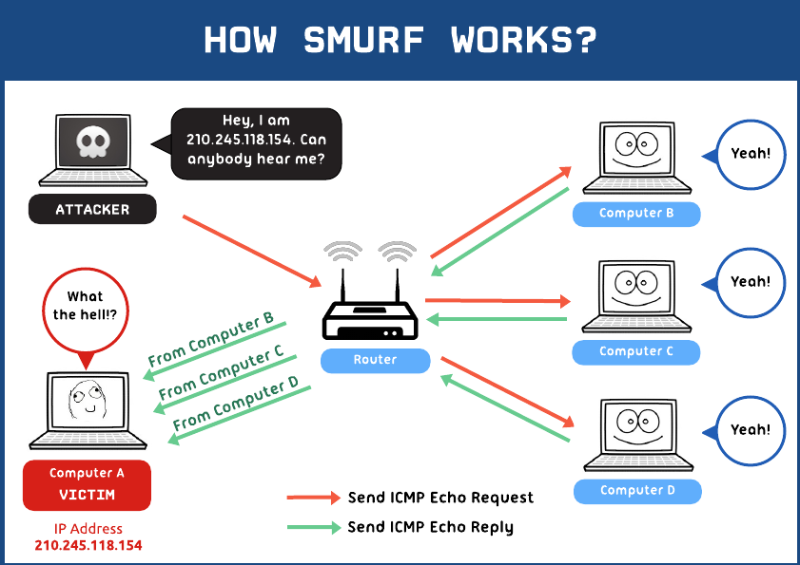
\includegraphics[width=\textwidth]{smurf}
					\caption{Schema di Smurf attack}
					\label{fig:smurf}
				\end{center}
			\end{figure}		
			Tutti questi messaggi andranno a saturare la rete della vittima che non potrà più usarla in alcun modo.
			
			Un attacco Neptune si basa su una cattiva configurazione di un server in attesa di connessioni. Per creare una connessione, un utente deve mandare prima un messaggio per richiedere il collegamento, aspettare una risposta positiva dal server e infine mandare una conferma di ricevuta risposta. Questo procedimento si chiama \emph{three-way handshake} (Figura \ref{fig:3way}). Le connessioni stabilite vengono poi salvate dal server su una tabella delle connessioni.
			\begin{figure}
				\begin{center}
					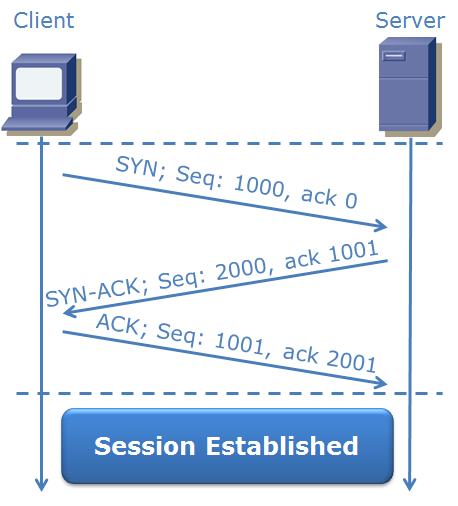
\includegraphics[width=.4\textwidth]{3wayh}
					\caption{Neptune attack}
					\label{fig:3way}
				\end{center}
			\end{figure}
			Quello che fa un attaccante è mandare il primo pacchetto ma non mandare mai il terzo lasciando il server in attesa di effettuare la connessione senza mai potersi liberare.
			
		\subsubsection{Attacchi di tipo Network Probe}
		Gli attacchi di questo tipo sono molto più semplici. Quelli che andremo ad approfondire sono il PortSweep e l'IPSweep.
		
		Ogni computer connesso ad una rete è raggiungibile attraverso un indirizzo chiamato indirizzo IP. Un attacco di IPSweep non fa altro che cercare sequenzialmente tutti gli IP connessi ad una rete. Una volta trovati gli indirizzi IP, per ognuno di questi esegue un PortSweep cioè una scansione sequenziale di tutte le porte di comunicazioni accessibili su ogni computer. Il grosso problema nel riconoscimento di questo tipo di attacchi è che a volte la scansione della rete o delle porte di un computer vengono eseguite legittimamente dagli amministratori di sistema per necessità di manutenzione o di controllo e quindi non possono essere impedite a priori.
		
	\subsection{Analisi dei dati}
		I dati per effettuare lo studio sono presi dal "1998 DARPA Intrusion Detection Evaluation data sets" e contiene dati di utilizzo della rete in sette settimane in caso di traffico normale e in caso di vari attacchi (tra i quali quelli di nostro interesse).
		
		\subsubsection{Preprocessing dei dati}
			Il dataset è stato preprocessato andando ad estrarre soltanto le informazioni riguardanti le intestazioni ("header") dei pacchetti passati dalla rete.
			Queste intestazioni sono divise in 12 parti (che saranno le nostre variabili).
			\begin{itemize}
				\item IPSource - IP mittente diviso in 4 parti (un generico indirizzo IP può essere 192.168.1.1)
				\item SPort - Porta di comunicazione del mittente
				\item IPDest - IP destinatario diviso in 4 parti
				\item DPort - Porta di comunicazione del destinatario
				\item Prot - Protocollo di comunicazione utilizzato
				\item Dim - Dimensioni del pacchetto
			\end{itemize}
			Sono stati creati 7 dataset, uno per ognuno dei quattro attacchi e tre per il normale traffico di rete (per cercare di comprendere diversi utilizzi benigni della rete). Data la grande dimensione dello spazio delle variabili (12 dimensioni) è molto difficile capire le relazioni che possono esserci tra di loro. Per questo motivo verrà utilizzata la \ac{PCA} con la prima e la seconda componente che descriveranno la maggior parte della varianza di qusti dati. Da notare che le prime due componenti forniscono solamente la direzione della massima varianza ma non forniranno una chiara indicazione sulla malignità/benignità del traffico ma i coefficienti della trasformazione (loading) ci forniranno questa indicazione.
			
	\subsection{Risultati}
		Come accennato, i \emph{principal component loading} sono i coefficienti della trasformazione delle componenti principali. Forniscono informazioni su quanto una certa variabile influisce sulla relativa componente principale. Un coefficiente alto indicherà che quella variabile ha una forte influenza su quella componente principale e viceversa. Nel nostro caso ci focalizzeremo sulle prime due componenti principali e sui relativi loadings (specialmente sulla variabile con il loading più alto).
		\begin{figure}
			\begin{center}
				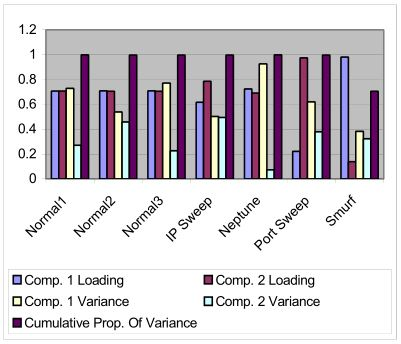
\includegraphics[scale=.8]{grafico}
				\caption{Loading e varianza delle componenti}
				\label{fig:grafico}
			\end{center}
		\end{figure}
		Nella Figura \ref{fig:grafico} possiamo vedere i due loadings più grandi in valore assoluto (SPort e DPort) e la varianza delle prime due componenti nei sette dataset.
		
		\subsubsection{Rilevare le intrusioni}
			L'idea fondamentale è la seguente. Come si vede dal grafico in Figura \ref{fig:grafico} i valori dei loadings delle prime due componenti principali in caso di traffico regolare sono quasi uguali mentre in caso di attacco differiscono considerevolmente (meno nell'attacco Neptune). Si potrebbe pensare di sfruttare questa conoscenza per riconoscere gli attacchi. Se i valori dei due loadings differiscono più di una certa soglia, facciamo scattare l'allarme. 
			
			A seconda della grandezza di questa soglia si può avere un comportamento più "difensivo" facendo scattare falsi allarmi in caso, ad esempio, di traffico benigno straordinario (manutenzione, nuovi incarichi temporanei,\dots ) o un comportamento un po' più "permissivo" magari perdendosi qualche attacco Neptune.
			
			Un secondo livello di analisi potrebbe però essere fatto sula varianza. Si può notare infatti che l'attacco di tipo Neptune ha come caratteristica una enorme differenza sulla varianza delle due componenti. Si può quindi pensare di affinare il rilevamento utilizzando due livelli. Se i loadings delle due componenti differiscono di molto dalla soglia, facciamo scattare l'allarme. Se sono vicini alla soglia controlliamo anche la varianza delle due componenti che, in caso di grandissima differenza, potrebbero suggerire un traffico malevolo.
		
\newpage
\section{Codice Python completo}
	\lstinputlisting[firstline=1, lastline=59]{code/PCA.py}
	\newpage
	\lstinputlisting[firstline=61, lastline=126]{code/PCA.py}
	\newpage
	\lstinputlisting[firstline=128, lastline=174]{code/PCA.py}

%----------------------------------------------------------------------------------------
%	BIBLIOGRAPHY
%----------------------------------------------------------------------------------------

%\begin{thebibliography}{99} % Bibliography - this is intentionally simple in this template
%
%\bibitem[Figueredo and Wolf, 2009]{Figueredo:2009dg}
%Figueredo, A.~J. and Wolf, P. S.~A. (2009).
%\newblock Assortative pairing and life history strategy - a cross-cultural
%  study.
%\newblock {\em Human Nature}, 20:317--330.
% 
%\end{thebibliography}

%----------------------------------------------------------------------------------------

\end{document}